\documentclass[12pt]{exam}

\usepackage[brazil]{babel}
\usepackage{enumerate}
\usepackage[utf8]{inputenc}
\usepackage{graphicx}

\extraheadheight{3cm}
\extrafootheight{2cm}
\extrawidth{2cm}
\headrule
\lhead {Universidade Estadual de Campinas 
    \\ Instituto de Computação 
    \\ \bfseries MO620 - Engenharia de Software II - Turma B 
    \\ \textnormal{Aluno: Luiz Alberto Ferreira Gomes}}
\rhead{
    Exercícios do Cap. 1: Introdução 
    \\  RA:007275}
\footrule
\footer{}{Página \thepage\ of \numpages}{}
\renewcommand{\solutiontitle}{\noindent\textbf{Solução:}\enspace}

\printanswers

\begin{document}
  \begin{questions}
    \question Explique e contraste cada um dos seguintes partes de termos: (i) instância e classe; (ii) comportamento e estado; (iii) agregação e herança; 
    (iv) herança e delegação.  
    \begin{solution}
      \begin{enumerate}[(i.)]
       \item \textbf{Instância e classe}: Uma classe é uma descrição de um molde que especifica as propriedades e o comportamentos relativos a um objetos similares. Uma instância 
	é uma ocorrência ou um objeto de uma classe. Os atributos e comportamentos são descritos, apenas uma vez, na classe e as instâncias derivam o seu estado e
	comportamento a partir dessa abstração que reúne as características e comportamentos comuns a diversos objetos.
       \item \textbf{Comportamento e estado}: O estado representa os valores que os atributos de um objeto assumem em um determinado instante durante o seu ciclo de vida. 
	O comportamento, por sua vez, representa suas operações que são implementadas através de métodos. Em OO o estado de um objeto é alterado através da invocação 
	de operações para um objeto alvo.
       \item \textbf{Agregação e herança}: A agregação é relacionamento "todo-parte" entre objetos de classes que possibilita criar hierarquias que representam uma abstração 
	a partir das partes que a compõe. O fato de cada parte poder possuir seus próprios componentes, possibilita uma refatoração recursiva. A herança é um relacionamento "é-um-tipo-de" 
	entre classes (em contraste com a agregação). Em hierarquias desse tipo, as características de uma categoria podem ser "herdadas" por outras, possibilitando a 
	existência de categorias genéricas (comuns) ou específicas. 
       \item \textbf{Herança e delegação}: A herança é um mecanismo de que permite o reúso em hierarquias de generalização/especialização, os atributos e operações são herdadas" das
        classes genéricas.A delegação, por sua vez, permite o reúso em hierarquias "todo-parte". O objeto "todo" pode reutilizar o comportamento  das suas "partes" por meio da invocação das suas operações.
	de agregação.
      \end{enumerate}
    \end{solution}

    \question 
      Dê um exemplo de duas hierarquias: uma de generalização/especialização e outra de agregação/ decomposição. Descreva as 
      diferenças e similaridades entre as duas hierarquias.
    \begin{solution}
      \begin{center}
	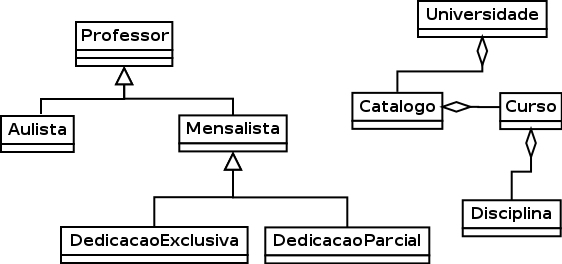
\includegraphics[width=.5\textwidth]{./exercicios-capitulo1-e2.png}
      \end{center}
      
      Enquanto a generalização/especialização é um relacionamento entre classes; a agregação/ decomposição é um relacionamento entre objetos. Ambas promovem o reúso de código, mas de forma diferente. A generalização/especialização por meio da herança e a agregação/decomposição por meio da delegação.
      
      
    \end{solution}
    
    \question 
      Construa uma hierarquia que represente os diversos tipos de contas disponíveis para os clientes do seu banco. Lembre-se
      de representar as classe mais genérica, denominada de \verb!ContaBancaria!.
      \begin{solution}
	\begin{center}
	  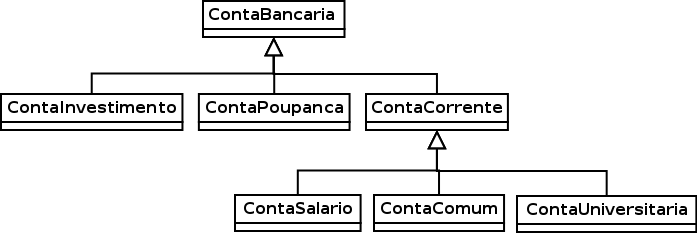
\includegraphics[width=.7\textwidth]{./exercicios-capitulo1-e3.png}
	\end{center}
      \end{solution}    
    
    \question 
      Defina atributos e operações para o tipo abstrato de dados \verb!CarteiraDeDinheiro!. Pense a respeito do comportamento de uma
      carteira e sobre os atributos relacionados com esse comportamento.
      \begin{solution}
	\begin{center}
	  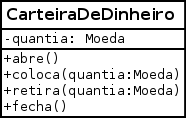
\includegraphics[width=.6\textwidth]{./exercicios-capitulo1-e4.png}
	\end{center}
      \end{solution}

    \question
      Defina uma classe representando uma pessoa com os seguintes atributos: nome, ano de nascimento e altura (em metros). Defina operações para 
      a iniciação desses atributos. Adicione uma operação que retorna a idade aproximada de uma pessoa de acordo com um determinado ano de de entrada.
      Adicione outra operação que retorna sua altura em centímetros.
      \begin{solution}
	\begin{center}
	  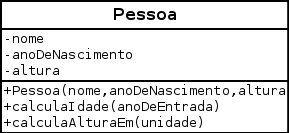
\includegraphics[width=.6\textwidth]{./exercicios-capitulo1-e5.png}
	\end{center}
      \end{solution}
    
    \question 
      Defina um classe para um tipo abstrato de dados ItemDeEstoque. Ela deve conter os atributos do nível de estoque e preço unitário. Defina métodos para 
      consultar os valores desses atributos e também para iniciá-los usando parâmetros. Adicione mais dois métodos para permitir a atualização do nível
      de estoque.
      \begin{solution}
	\begin{center}
	  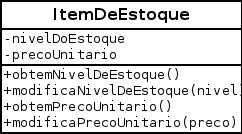
\includegraphics[width=.6\textwidth]{./exercicios-capitulo1-e6.png}
	\end{center}
      \end{solution}
    
    \question 
      Suponha que você esteja desenvolvendo uma classe que represente um baralho de cartas. Quais operações você deveria oferecer na interface pública 
      da classe? Faria sentido você modelar essa abstração usando duas classes separadas: uma para modelar o baralho e outra para representar as cartas?
      Por quê?
      \begin{solution}
      
        A classe deveria oferecer as operações: embaralhar, colocar(carta) e retirar(carta). Sim, pois um baralho é composto de cartas. Isso poderia ser modelado utilizando a agregação/decomposição.
        \begin{center}
	       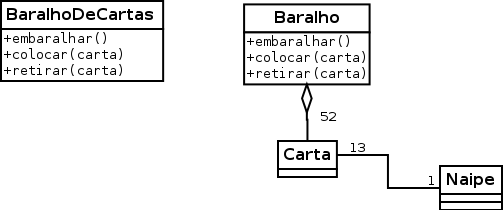
\includegraphics[width=.8\textwidth]{./exercicios-capitulo1-e7.png}
        \end{center}
      \end{solution}

      \question 
        Para os diagramas da classe da figura abaixo, discuta os "erros"  de modelagem cometidos (caso eles existam) e proponha soluções corretivas.

        \begin{center}
	       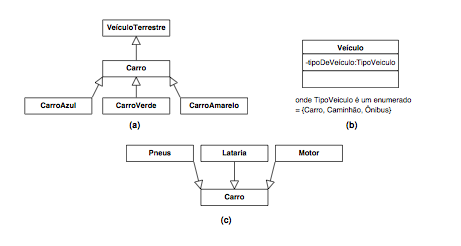
\includegraphics[width=.8\textwidth]{./figura-com-erros-de-modelagem.png}
        \end{center}
      
        \begin{solution}
          \begin{enumerate}[(i.)]
           \item \textbf{na situação (a)}, as classes CarroAzul, CarroVerde e CarroAmarelo não tipificam especializações de um carro, mas sim a característica cor
            desse tipo de veículo. A cor deveria ser modelada como um atributo da classe Carro.
           \item \textbf{na situação (b)}, o tipo de veículo poderia ser melhor modelado criando-se uma hierarquia com as especializações de veículo
           como Carro, Caminhão e Ônibus.
           \item \textbf{na situação (c)}, Pneus, Lataria e Motor são partes de um carro e não especializações como mostra a figura.
           \end{enumerate}
        \end{solution}

      \question 
        Crie uma hierarquia de generalização/especialização que modele os alimentos encontrados nas prateleiras de um supermercado. Identifique 
        atributos associados a cada uma das classes.
        \begin{solution}
          \begin{center}
            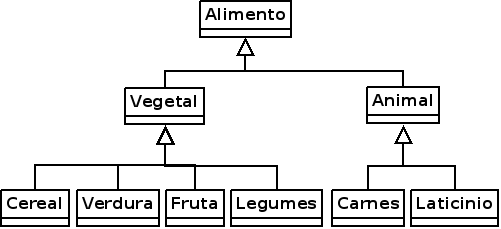
\includegraphics[width=.8\textwidth]{./exercicios-capitulo1-e9.png}
          \end{center}
        \end{solution}

      
      \question 
      Crie um modelo de objetos que represente um carro que possa ser colocado e retirado de uma garagem. Quantas abstrações você acha que são
      necessárias para o modelo represente o mais fielmente possível a realidade? Quais operações você poderia oferecer na interface pública das
      classes usadas?
        \begin{solution}
          \begin{center}
            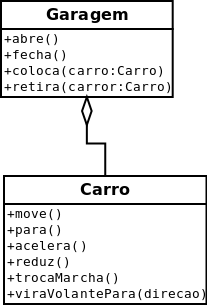
\includegraphics[width=.3\textwidth]{./exercicios-capitulo1-e10.png}
          \end{center}
        \end{solution}
      
      \question 
      Defina uma hierarquia de classes que represente um coleção de números. Uma coleção é um grupo de objetos. Um conjunto é um tipo de coleção
      onde não existem duplicatas e uma lista é uma coleção onde seus elementos estão ordenados. Identifique o comportamento de cada tipo abstrato de dados envolvido na modelagem.
        \begin{solution}
          \begin{center}
            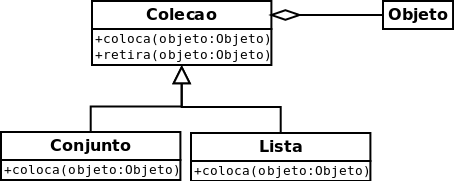
\includegraphics[width=.5\textwidth]{./exercicios-capitulo1-e11.png}
          \end{center}
        \end{solution}
        
      \question 
      Modele uma hierarquia de classe parcial para um sistema de controle de reservas e ocupações em um hotel. O hotel é constituído por um conjunto de quartos (simples e duplos), auditórios para conferências e salões de festas. O sistema controla a ocupação e desocupação do seus cômodos, bem como, permite que o usuário verifique o estado atual de cada cômodo, isto é, se ele está ocupado ou desocupado.
        \begin{solution}
          \begin{center}
            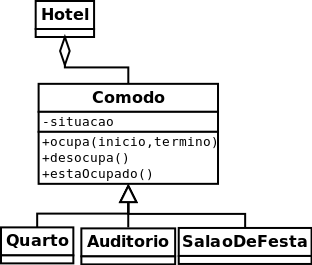
\includegraphics[width=.5\textwidth]{./exercicios-capitulo1-e12.png}
          \end{center}
        \end{solution}
      
      \question 
      Classifique e crie uma hierarquia de generalização/especialização contendo os diferentes tipos de itens encontrados na biblioteca de uma universidade. Sugestão: livros, periódicos, teses, fitas  de vídeo, DVD etc. Identifique atributos e as operações de cada tipo abstrato de dados.
        \begin{solution}
          \begin{center}
            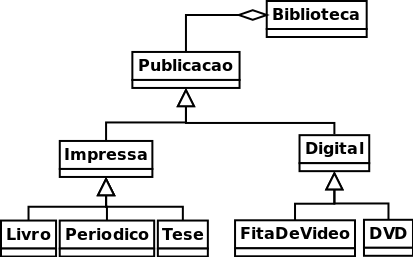
\includegraphics[width=.5\textwidth]{./exercicios-capitulo1-e13.png}
          \end{center}
        \end{solution}
      
  \end{questions}

\end{document}
